
\subsection{Ausgangslage}
Der Einsatz von Fadenwürmern ist im Gartenbau verbreitet. Konventionell werden Nematoden in Wasser aufgelöst und durch ein Dosiergerät oder eine Spritzkanne in Pflanzennähe aufgetragen \cite{birchmeier}. Solche Produkte werden jedoch erst bei erhöhtem Befall von Schädlingen eingesetzt. Die Firma MCC Laboratoire Meiners GmbH verfolgt einen anderen Ansatz. Präventiv möchten Sie Nematoden in Topfpflanzen einsetzen. Topfpflanzen sollen so, bereits bestückt mit NemaCaps, im Detailhandel angeboten werden. 
\subsubsection{Topfmaschine}
\begin{wrapfigure}[15]{r}{10cm}
	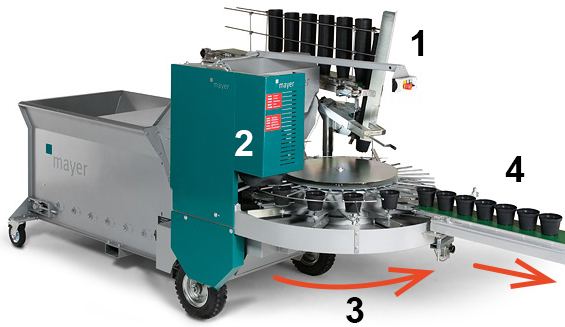
\includegraphics[draft=false,scale=0.5]{Illustrationen/3-Einleitung/schema_topfmaschine.jpg}
	\caption{Topfmaschine \protect\cite{mayer}}
	\label{fig:schema_topfmaschine}
\end{wrapfigure}
Das industrielle Eintopfen von Topfpflanzen wird heute unter anderem mit halbautomatischen Topfmaschinen erledigt. In getakteten Schritten werden Töpfe mit einem minimalen manuellen Eingriff mit Jungpflanzen (sogenannten Setzlingen) bestückt. In einem Magazin werden leere Töpfe gelagert (Punkt 1 in Abbildung \ref{fig:schema_topfmaschine}). Diese Töpfe fallen getaktet auf einen rotierenden Topfkranz. Im Gegenuhrzeigersinn werden die leeren Töpfe zur Schütte bewegt (2). Dort wird der Topf mit Erde befüllt, ein Loch gebohrt und die überschüssige Erde abgetragen. Der befüllte Topf rotiert nun zu Punkt 3, wo ein Arbeiter den Setzling manuell ins gebohrte Loch eintopft. Der Topfkranz rotiert das fertige Produkt zu Punkt 4 wo es auf ein Förderband umgeleitet wird und die Prozesskette der Topfmaschine verlässt.

